\documentclass{homework}
\usepackage{cancel}
\usepackage{amsthm}
\usepackage{cleveref}
\usepackage{upgreek}
\usepackage[framed]{mcode}
\usepackage{mathrsfs}
\usepackage{tikz}
\usepackage{units}
\usetikzlibrary{matrix}
\newtheorem{lemma}{Lemma}
\DeclareMathOperator*{\argmin}{arg\,min}

\title{Kevin Joyce}
\course{Math 514 - Inverse Problems - Homework 3}
\author{Kevin Joyce}
\docdate{\today}
\begin{document} 
\newcommand{\figref}[1]{\figurename~\ref{#1}}
\renewcommand{\bar}{\overline}
\renewcommand{\hat}{\widehat}
\renewcommand{\SS}{\mathcal S}
\newcommand{\HH}{\mathscr H}
\newcommand{\mom}{\widetilde}
\newcommand{\mle}{\widehat \Uptheta}
\newcommand{\eps}{\varepsilon}
\newcommand{\todist}{\stackrel{D}\longrightarrow}
\newcommand{\toprob}{\stackrel{p}\longrightarrow}
\newcommand{\TTheta}{\overline{\underline \Theta} }
\newcommand{\del}{\partial}
\newcommand{\approxsim}{\overset{\cdotp}{\underset{\cdotp}{\sim}}}

\begin{longproblem} 
Bardsley 2.1.

\subproblem{ Recall the minimization problem for Tikhonov regularization, 
\begin{equation}
  \vect x_{\alpha} = \argmin_{\vect x} \left\{ \frac 12 \| \vect{Ax} - \vect
  b\|^2 + \frac\alpha 2\| \vect x\|^2 \right\}.\tag{2.5} \label{2.5}
\end{equation}
Define $\ell(x)$ to be the penalized least squares function and
show that $\nabla \ell(\vect x) = \vect 0$ yields
\begin{equation}
  (\vect A^T \vect A + \alpha \vect I)\vect x = \vect A^T \vect b\tag{2.6} \label{2.6}
\end{equation}
and hence that solution of \eqref{2.5} and \eqref{2.6} coincide.  Argue, moreover, that the solution is unique. }
\begin{solution}
  Expanding $\ell(x)$ and denoting the  inner product between two vectors as $\vect x \cdot \vect y$, we have
  \begin{align*}
    2 \ell(\vect x) &= (\vect{Ax} - \vect b)^T (\vect{Ax} - \vect b) + \alpha \vect x^T \vect x\\
    &= \vect x^T (\vect A^T \vect A + \alpha \vect I)\vect x -\vect b^T\vect{Ax} - \vect x^T (\vect A^T\vect b) + \vect b^T\vect b\\
    &= \vect x^T (\vect A^T \vect A + \alpha \vect I)\vect x - 2\vect x \cdot (\vect A^T \vect b) + \vect b^T\vect b\quad\text{ by symmetry of real inner products.}\\
  \end{align*}
  We evaluate the gradient $2\ell(\vect x)$ term by term.  The gradient of the constant $\vect b^t \vect b$ is $\vect 0$, and the gradient of the vector function $\vect x \to \vect x \cdot (\vect A^T \vect b)$ is precisely $\vect A^T \vect b$. Note that the quadratic form $f(\vect x) = \vect x^T(\vect A^T\vect A + \alpha \vect I)\vect x$ has
  \begin{align*}
  f(\vect x + \vect h) - f(\vect x) 
  &= (\vect x + \vect h)^T (\vect A^T \vect A + \alpha \vect I)(\vect x + \vect h) - \vect x^T (\vect A^T \vect A + \alpha \vect I)\vect x\\
  &= \vect h^T (\vect A^T \vect A + \alpha \vect I)\vect x +\vect x^T(\vect A^T \vect A + \alpha \vect I)\vect h + \vect h^T (\vect A^T \vect A + \alpha \vect I)\vect h\\
%  &= 2 \vect h^T (\vect A^T \vect A + \alpha \vect I)\vect x + \vect h^T (\vect A^T \vect A + \alpha \vect I)\vect h\\
  &= 2 \vect h \cdot \Big[ (\vect A^T \vect A + \alpha \vect I)\vect x + (\vect A^T \vect A + \alpha \vect I)\vect h\Big ]\quad\text{ by symmetry.}\\
  \end{align*}
  Note that if $\nabla f(\vect x) = 2(\vect A^T \vect A + \alpha \vect I)\vect x$, then 
$$
  \lim_{\|\vect h\| \to 0} \frac{\|f(\vect x + \vect h) - f(\vect x) - \vect h \cdot \nabla f\|}{\|\vect h\|} = 
  \lim_{\|\vect h\| \to 0} \frac{\|\vect h^T (\vect A^T\vect A + \alpha\vect I)\vect h\|}{\|\vect h\|} = 0  
$$
by Cauch-Schwartz applied twice.
Hence, $\nabla \ell (\vect x) = 0$ if and only if
$$
   (\vect A^T \vect A + \alpha \vect I)\vect x - \vect A^T \vect b  + \vect 0 = \vect0 \iff (\vect A^T \vect A + \alpha \vect I)\vect x = \vect A^T \vect b.
$$
Recall that the singular
value decomposition of $\vect A =  \vect{U \Sigma}\vect V^T$ is such that
the diagonal elements of $\vect \Sigma$ are each non-negative real numbers. Moreover, if $\alpha > 0$, then $\vect A^T\vect A + \alpha \vect I = \vect V(\vect \Sigma^T\vect\Sigma + \alpha\vect I)\vect V^T$ is an eignvalue decomposition with each eigenvalue strictly greater than 0 if and only if $\vect A^T \vect A + \alpha \vect I$ has full rank if and only if the solution to the matrix equation above is unique.

\end{solution}

\subproblem{ Use the SVD of a matrix $\vect A$ to show that the solution of \eqref{2.6} (and hence \eqref{2.5}) can be written in filtered SVD form
\begin{equation}
  \vect x_{\alpha} = \vect V \vect \Phi_\alpha \vect \Sigma^\dagger \vect U^T \vect b\tag{2.3} \label{2.3}
\end{equation}
with Tikhonov filter 
\begin{equation}
  \vect \Phi _\alpha = \mathrm{diag}\left( \frac{\sigma_1^2}{\sigma_1^2 + \alpha} , \dots, \frac{\sigma_n^2}{\sigma_n^2 + \alpha}\right) .\tag{2.7} \label{2.7}
\end{equation}}

\begin{solution}
  Let $\vect A = \vect{U\Sigma V}^T$, then the Tikhonov solution is given by
  \begin{align*}
  \vect v_\alpha 
  &= (\vect A^T \vect A - \alpha \vect I)^{-1} \vect A^T \vect b\\
  &= (\vect V \vect \Sigma^T\vect \Sigma \vect V^T - \alpha \vect V\vect V^T)^{-1} \vect V\vect \Sigma^T \vect U^T \vect b\\
  &= \vect V (\vect \Sigma^T\vect \Sigma  - \alpha \vect I)^{-1}\cancel{\vect V^T \vect V}\vect \Sigma^T\vect I \vect U^T \vect b\\
  &= \vect V (\vect \Sigma^T\vect \Sigma  - \alpha \vect I)^{-1}\vect\Sigma^T (\vect\Sigma \vect \Sigma^\dagger) \vect U^T \vect b\\
  &= \vect V \vect \Phi_{\alpha} \vect \Sigma^\dagger\vect U^T \vect b.\\
  \end{align*}
  since $\vect \Sigma^T\vect \Sigma$ and  $\alpha \vect I$ are both $n\times n$ a diagonal matrices with diagonal elemenst $\sigma_i^2$ and $\alpha$ respectively, and $\vect \Sigma^\dagger$ is a right inverse for the matrix $\vect \Sigma$. 
  \end{solution}
\end{longproblem}

\problem{Bardsley 2.2.a. Create plots of the \emph{relative error} function $f(\alpha) = \|\vect x_\alpha - \vect x_{\mathrm{true}}\| / \|\vect x_{\mathrm{true}}\|$ within both \texttt{DeblurTikhonov.m} and \texttt{PSFReconTikhonov.m} (use MATLAB's \texttt{logspace} function).  Then estimate from the plots which $\alpha$ minimizes the relative error.}
\begin{solution}
\begin{center}
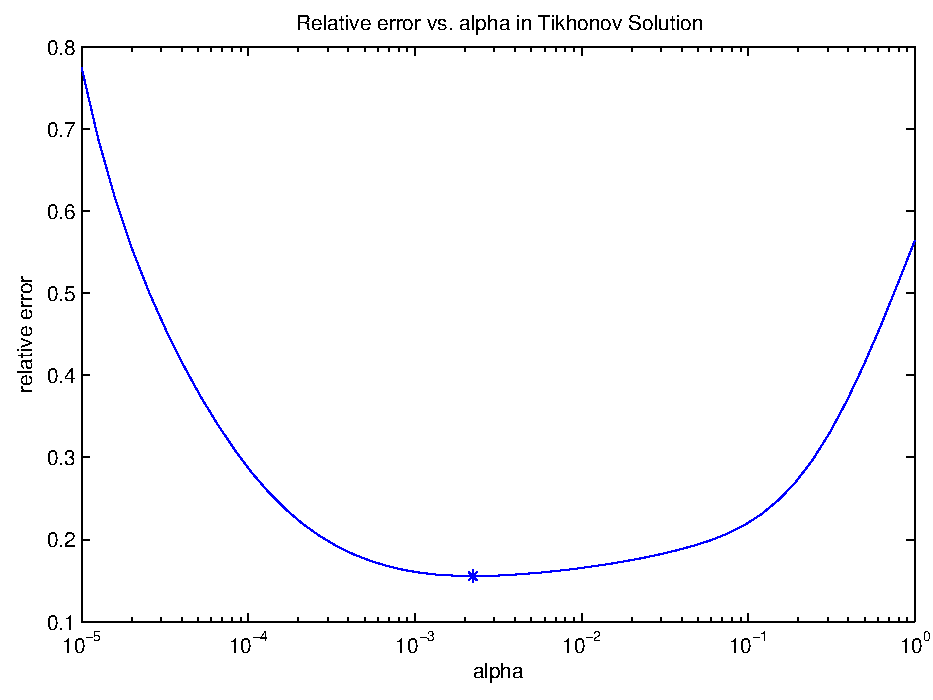
\includegraphics[width=.4\textwidth]{rel_error_tikhonov.pdf}
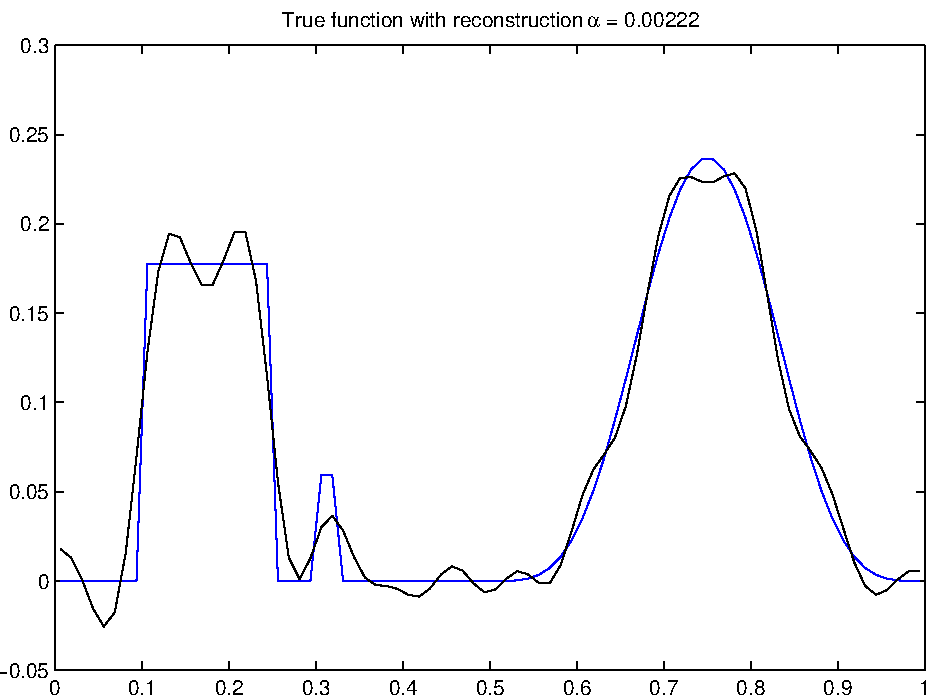
\includegraphics[width=.4\textwidth]{opt_rel_error_tikhonov.pdf}
\end{center}
\begin{center}
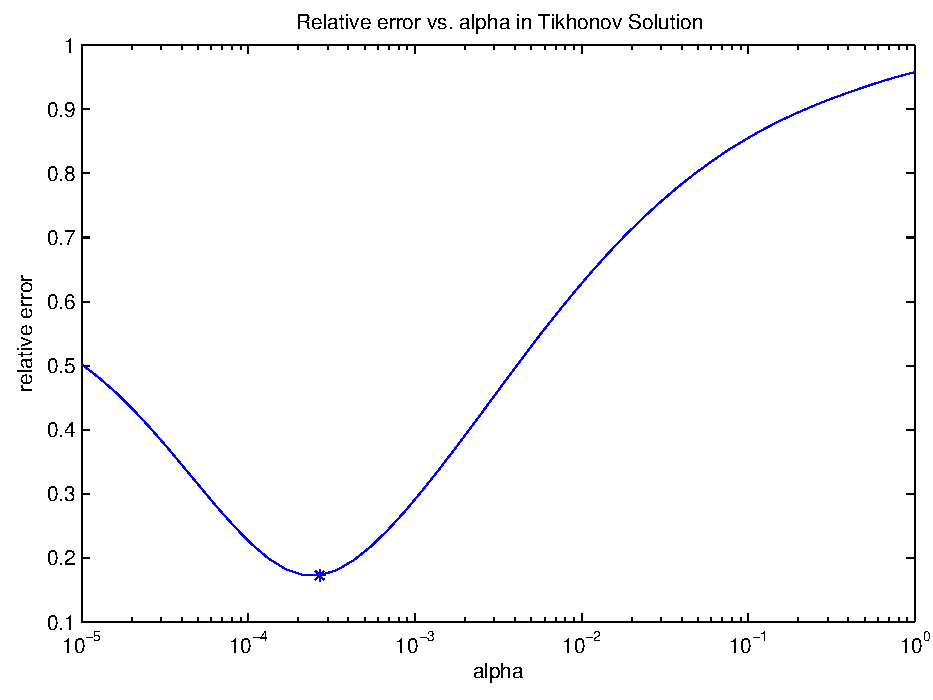
\includegraphics[width=.4\textwidth]{psf_rel_error.pdf}
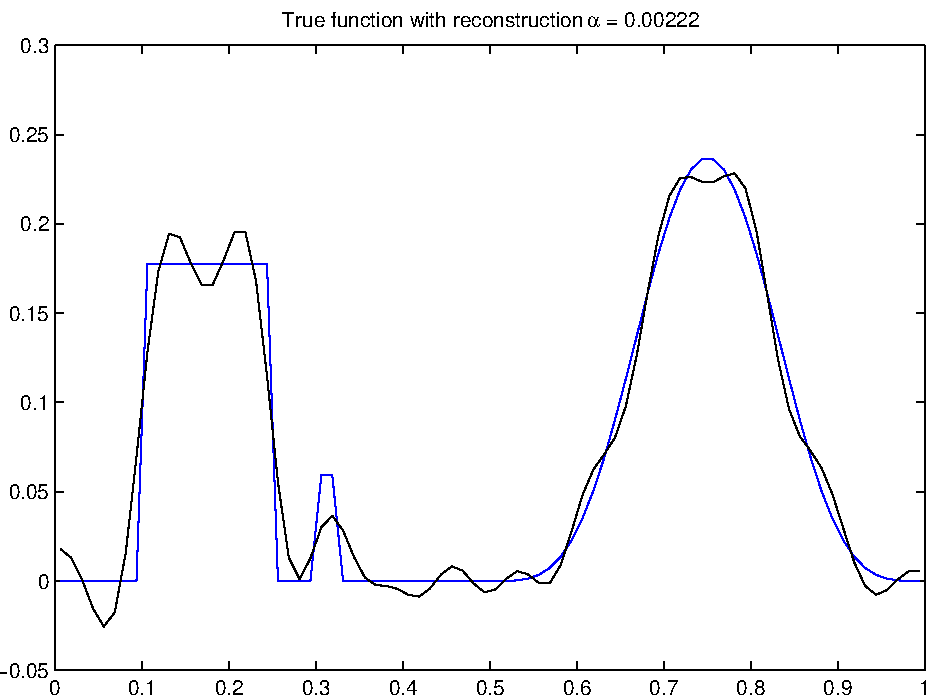
\includegraphics[width=.4\textwidth]{psf_rel_error_solution.pdf}
\end{center}
\end{solution}

\begin{longproblem}Bardsley 2.5.a \& b 

\subproblem{Find the expressions for the MSE defined by 
\begin{equation}
\mathrm{MSE}(\nu) = \sigma^2\sum_{i=1}^n(\phi_i^{(\nu)}/\sigma_i)^2 + \sum_{i=1}^n (1 - \phi_i^{(\nu)} )^2 (\vect v_i^T \vect x)^2.\tag{2.14}\label{2.14}
\end{equation}
for the TSVD, Tikhonov, and Landweber regularized solutions.}

\begin{solution}
  In the case of TSVD, recall that the filter operator is the projection onto the first $k$ singular vectors $v_1,\dots,v_k$.  So $\phi_i^{(k)} = 1$ if $i \le k$ and $0$ otherwise; hence,
  $$
    \mathrm{MSE}(k) =\sigma^2\sum_{i=1}^k\sigma_i^{-2} + \sum_{i=k+1}^n (\vect v_i^T \vect x)^2 
  $$

  For Tikhonov regularization, $\phi_i^{(\alpha)} = \sigma_i^2/(\sigma_i^2 + \alpha)$.  Substituting into \eqref{2.14},
  $$
    \mathrm{MSE}(\alpha) = \sigma^2\sum_{i=1}^n\left(\frac{\sigma_i}{\sigma_i^2 + \alpha}\right)^2 + \sum_{i=1}^n \left( \frac{\alpha}{\sigma_i^2 + \alpha}\right)^2 (\vect v_i^T \vect x)^2.
  $$

  For Landweber, recall $\phi_i^{(n,\tau)} = 1 - (1 - \tau \sigma_i^2)^n$ for $n=1,2,\dots$ and $0<\tau<1/\sigma_1$. Hence,
  \begin{align*}
    \mathrm{MSE}(n,\tau) &= \sigma^2\sum_{i=1}^n(\sigma_i^{-1}(1 - (1 - \tau\sigma_i^2)^n)^2 + \sum_{i=1}^n (1 - \tau \sigma_i^2)^{2n} (\vect v_i^T \vect x)^2\\
    &= \sigma^2\sum_{i=1}^n\left(\tau \sigma_i \sum_{k=0}^{n-1}(1-\tau\sigma_i^2)^k\right)^2 + \sum_{i=1}^n (1 - \tau \sigma_i^2)^{2n} (\vect v_i^T \vect x)^2.\\  \end{align*}
\end{solution}

\subproblem{Create plots of $\mathrm{MSE}(\alpha)$, using MATLAB's \texttt{logspace} function, within both \texttt{DeblurTikhonov.m} and \texttt{PSFreconTikhonov.m}.  Then estimate from the plots which $\alpha$ minimizes the MSE.}

This problem was combined with the following one.

\end{longproblem}


\begin{longproblem}Bardsley 2.6.a \& d

\subproblem{ Modify \texttt{DeblurTikhonov.m} and \texttt{PSFreconTikhonov.m} so that (some subset of) the following curves are plotted together, (all on the same numerical grid created using \texttt{logspace}):}
\begin{enumerate}[i]
  \item the UPRE curve $U(\alpha)$ defined by 
  \begin{equation}
  U(\alpha) = \sum_{i=1}^b \frac{\alpha^2 (\vect u_i^T \vect b)^2}{(\sigma_i^2 + \alpha)^2} + 2\sigma^2 \sum_{i=1}^n \vect {\sigma_i^2}{\sigma_i^2 + \alpha}.\tag{2.21}\label{upre}
  \end{equation}
  \item the GCV curve $G(\alpha)$ defined by 
  \begin{equation}
  G(\alpha) = \left(\sum_{i=1}^n \frac{\alpha^2(\vect u_i^T \vect b)^2}{(\sigma_i^2 + \alpha)} \right) \left/ \middle( m - \sum_{i=1}^n\frac{\sigma_i^2}{\sigma_i^2 + \alpha} \right)\tag{2.25}\label{gcv}
  \end{equation}
  \item the DP curve $D(\alpha)^2$ defined by 
  \begin{equation}
  D(\alpha) = \sum_{i=1}^n \frac{\alpha^2 (\vect u_i^T \vect b)^2}{(\sigma_i^2 + \alpha)^2} - m\sigma^2 \tag{2.29}\label{dpcurve}
  \end{equation}
  \item the L-curve curvature function $-C(\alpha)$ defined by 
  \begin{equation}
  C(\alpha) = -\frac{r(\alpha) s(\alpha) [\alpha r(\alpha) + \alpha^2 s(\alpha) ] + [r(\alpha)s(\alpha)]^2/s'(\alpha)]}{[r(\alpha)^2 + \alpha^2 s(\alpha)^2]^{3/2}}\tag{2.37}\label{lcurve}
  \end{equation} 
  where $s(\alpha) = \|\vect x_\alpha\|^2$, and $r(\alpha) = \|\vect{Ax}_\alpha - \vect b\|^2$.
\end{enumerate}

\end{longproblem}

\enlargethispage{3em}
\begin{solution}
Minimums for each curve were estimated using MATLABs \texttt{fminbnd} function.  Note that each method selects a $\hat \alpha$ that is bounded above by those given by the MSE and relative error.

\begin{minipage}{.55\textwidth}
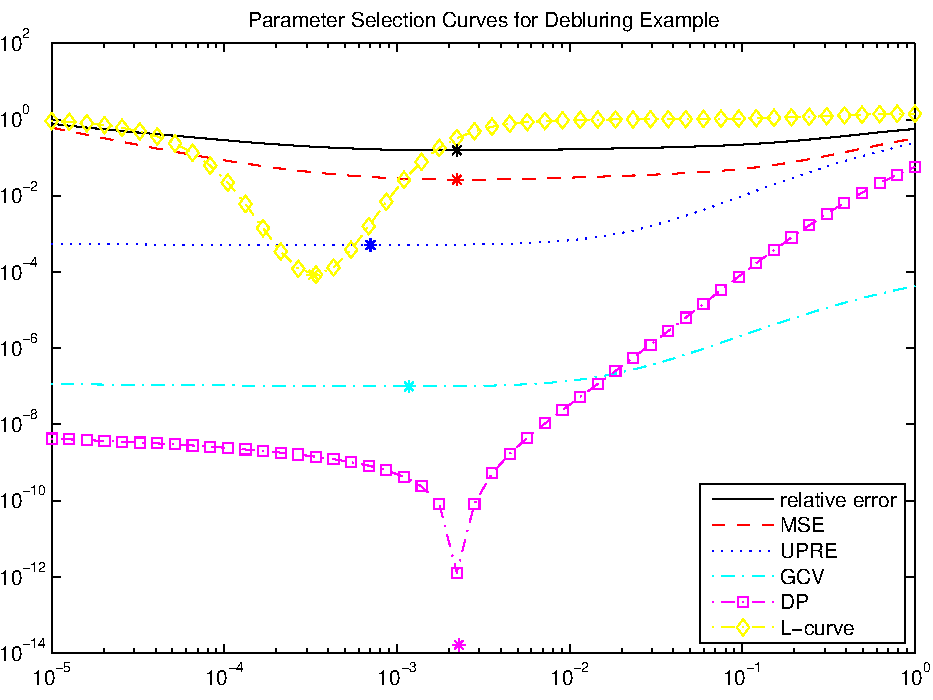
\includegraphics[width=\textwidth]{all_curves.pdf}
\end{minipage}
\begin{minipage}{.35\textwidth}
\begin{tabular}{ c c }
\hline
relative error & $\hat \alpha = 2.226\times 10^{-3}$\\
MSE & $\hat \alpha =     2.376\times 10^{-3}$\\
UPRE & $\hat \alpha =    7.024\times 10^{-4}$\\
GCV & $\hat \alpha =	    1.173\times 10^{-3}$\\
DP & $\hat \alpha =	    2.282\times 10^{-3}$\\
L-curve & $\hat \alpha = 3.271\times 10^{-4}$\\
\hline
\end{tabular}
\end{minipage}

\begin{minipage}{.55\textwidth}
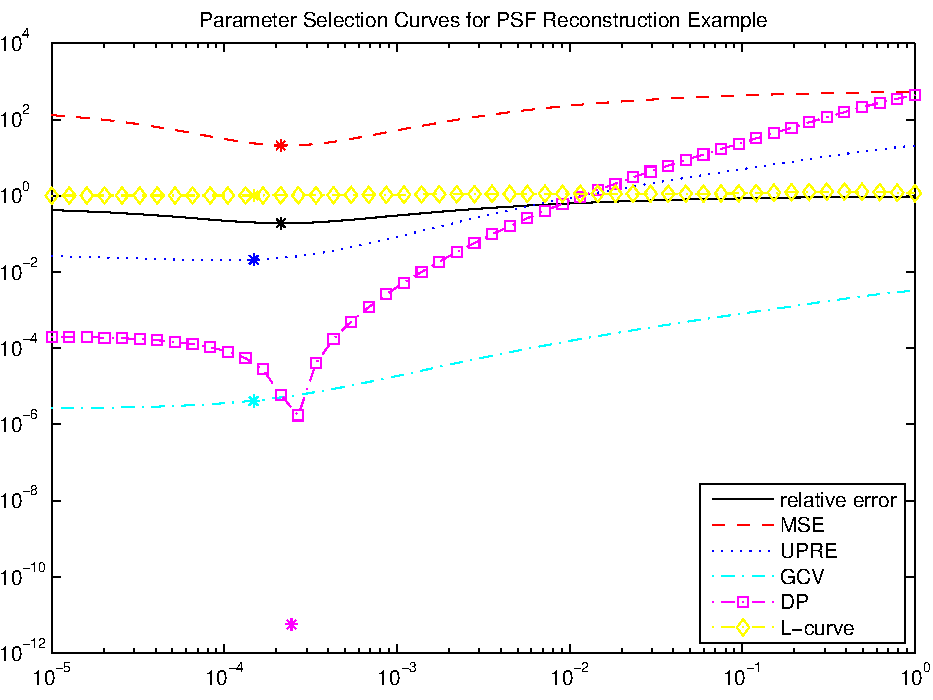
\includegraphics[width=\textwidth]{all_curves_psf.pdf}
\end{minipage}
\begin{minipage}{.35\textwidth}
\begin{tabular}{ c c }
\hline
relative error & $\hat \alpha = 2.518\times 10^{-4}$\\
MSE & $\hat \alpha = 2.185\times 10^{-4}$\\
UPRE & $\hat \alpha = 1.399\times 10^{-4}$\\
GCV & $\hat \alpha = 1.399\times 10^{-4}$\\
DP & $\hat \alpha = 1.828\times 10^{-4}$\\
L-curve & $\hat \alpha = 1.457\times 10^{-4}$\\
\hline
\end{tabular}
\end{minipage}
\end{solution}

\end{document} 
